\section{Lecture 18}
\subsection{Lecture Notes - Moment of Inertia Tensor}
\subsubsection{Review of Last Day's Results}
\[\v{L} = \v{L}_{CM} + \v{L}_{rel}\]
\[T = T_{CM} + T_{rel}\]
\[U = U_{CM} + U_{rel}\]
We can decompose the angular momentum and energies into the center of mass term and the relative to the COM term. We note that for rigid bodies, $U_{rel}$ is constant. 
\newline Last time (see 17.1.5) we observed that the angular momentum vector and the rotation vector are, in general, not parallel. Let us solve a question with a similar idea. Suppose we have a rotating dumbbell of two masses $m$ which move in circles (radius $a$) at a z displacement $l$ and $-l$, joined by a massless rod. The Angular velocity vector is given by $\bm{\omega} = \omega\zhat$. What is the direction of $\v{L}$?
\begin{center}
    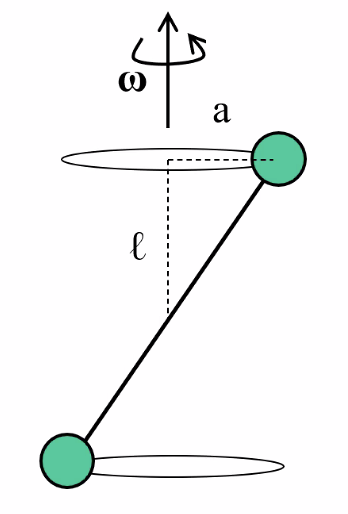
\includegraphics[scale=0.5]{Lecture-18/l18-img1.png}
    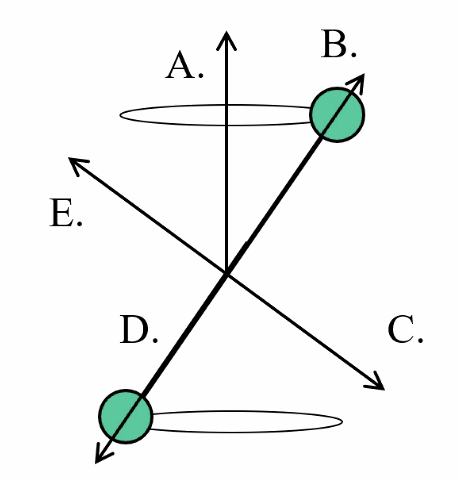
\includegraphics[scale=0.5]{Lecture-18/l18-img2.png}
\end{center}
\begin{s}
Direction E. Use the right hand rule with $\v{L} = \v{r} \times \v{v}$ and the add the angular momenta of the two terms.
\end{s}
Follow-up question; consider the body frame where the position of the masses are $(0, a, l)$, $(0, -a, -l)$. What is the $I_{zz}$ component of the inertia tensor?
\begin{s}
Recall that $I_{zz} = \sum_\alpha m_\alpha(x_\alpha^2 + y_\alpha^2)$. Applying the formula, we have that $I_zz = ma^2 + m(-a)^2 = 2ma^2$.
\end{s}
\noindent Next, what is the $I_{xz}$ component of the inertia tensor?
\begin{s}
Recall that $I_{xz} = -\sum_\alpha x_\alpha z_\alpha$. We see that $x = 0$ for both masses so hence $I_{xz} = 0$.
\end{s}
\noindent What's $I_{yz}$?
\begin{s}
Recall that $I_{yz} = -\sum_\alpha m_\alpha y_\alpha z_\alpha$. We therefore have that $I_{yz} = -mal - m(-a)(-l) = -2mal$.
\end{s}
\noindent What is the kinetic energy of the system?
\begin{s}
We use that $T = \frac{1}{2}I_{zz}\omega^2 = \frac{1}{2}(2ma^2)\omega^2 = ma^2\omega^2$.
\end{s}
\noindent \textit{Remark:} We can genrealize this to be $T = \frac{1}{2}\bm{\omega} \cdot \v{L}$.

\subsubsection{Angular momentum for rigid body with angular velocity along arbitrary direction}
We have that:
\[\bm{\omega} = \m{\omega_x \\ \omega_y \\ \omega_z}\]
As well as that:
\[\v{L} = \sum_\alpha m_\alpha \left(\v{r}_\alpha \times (\bm{\omega} \times \v{v}_\alpha)\right)\]
We apply the BAC-CAB rule, that is:
\[\v{A} \times (\v{B} \times \v{C}) = \v{B}(\v{A} \cdot \v{C}) - \v{C}(\v{A} \cdot \v{B})\]
Using this, the above expression for the angular momentum becomes:
\[\v{L} = \m{L_x \\ L_y \\ L_z} = \sum_\alpha m_\alpha \m{(y_\alpha^2 + z_\alpha^2)\omega_x & - x_\alpha y_\alpha \omega_y & -x_\alpha z_\alpha \omega_z
\\ -y_\alpha x_\alpha \omega_x & (z_\alpha^2 + x_\alpha^2)\omega_y & -y_\alpha z_\alpha \omega_z
\\ -z_\alpha x_\alpha \omega_x & -z_\alpha y_\alpha \omega_y & (x_\alpha^2 + y_\alpha^2)\omega_z}\]
We may pull out these coefficients and define a moment of inertia matrix/tensor:
\[\II = \m{I_{xx} & I_{xy} & I_{xz} \\ I_{yx} & I_{yy} & I_{yz} \\ I_{zx} & I_{zy} & I_{zz}}\]
Where $\v{L} = \II\bm{\omega}$. Note that this matrix is both real symmetric, as $I_{ij} = I_{ji}$, and hence contains 6 independent elements. We also note that this means $\II^T = \II$ (equal to its transpose). For example, using the definition, we can say that:
\[I_{xx} = \sum_\alpha m_\alpha(y_\alpha^2 + z_\alpha^2)\]
\[I_{xy} = -\sum_\alpha m_\alpha x_\alpha y_\alpha = -\sum_\alpha m_\alpha y_\alpha x_\alpha = I_{yx}\]
We can extend this notion to continuous mass distributions:
\[\II = \int dV\rho(x, y, z)\m{y^2 + z^2 & -xy & -xz \\ -xy & x^2 + z^2 & -yz \\ -xz & -yz & x^2 + y^2
}\]
\subsubsection{Index notation}
Note that when we write $\v{L} = \II\bm{\omega}$, this is equivalent to $L_i = \sum_j I_{ij}\omega_j$. We can also write this compactly by introducing the Kronecker Delta notation:
\[\delta_{ij} = \begin{cases}
1 & \text{if $i = j$}
\\ 0 & \text{otherwise}
\end{cases}\]
Hence we could write the above expression for the inertia tensor more compactly as:
\[I_{ij} = \int dV\rho(x,y,z)\left(\v{r}^2\delta_{ij} - r_ir_j\right)\]

\subsubsection{Example: Components of Inertia Tensor for rotation of cube about corner}
\begin{center}
    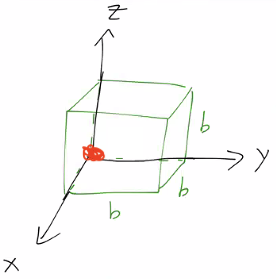
\includegraphics[scale=1]{Lecture-18/l18-img3.png}
\end{center}
We have a uniform solid cube of mass $M$ and side $b$, rotating about a corner (the origin). We assume a constant $\rho$ of $\rho = \frac{M}{b^3}$. Calculating $I_{xx}$, we have:
\[I_{xx} = \rho\int_0^bdx \int_0^bdy \int_0^bdz (y^2 + z^2) = \ldots = \frac{2}{3}Mb^2\]
Note we have pulled out $\rho$ from the integration as these are constant. By symmetry of the object, $I_{xx} = I_{yy} = I_{zz}$. What about the off diagonal terms? Calculating $I_{xy}$ we have:
\[I_{xy} = \rho\int_0^bdx\int_0^bdy\int_0^bdz(-xy) = -\frac{M}{4}b^4\]
And we would expect the other off diagonal elements to again be identical by symmetry. Writing the total inertia tensor, we then have:
\[\II = Mb^2\m{2/3 & -1/4 & -1/4 \\ -1/4 & 2/3 & -1/4 \\ -1/4 & -1/4 & 2/3}\]

\subsubsection{Example: Components of Inertia Tensor for rotation of cube about COM}
\begin{center}
    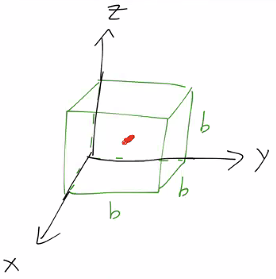
\includegraphics[scale=1]{Lecture-18/l18-img4.png}
\end{center}
Our bounds of integration will change compared to the last case. Calculating $I_{xx}$, we have:
\[I_{xx} = \rho\int_{-b/2}^{b/2}dz\int_{-b/2}^{b/2}dy\int_{-b/2}^{b/2}dz(y^2 + z^2) = \frac{Mb^2}{6}\]
Again by symmetry, $I_{xx} = I_{yy} = I_{zz}$. We note that this is different from before! Calculating $I_{xy}$, we have:
\[I_{xy} = \rho\int_{-b/2}^{b/2}dz\int_{-b/2}^{b/2}dy\int_{-b/2}^{b/2}dz(-xy) = 0\]
The integral is immediately zero by the fact that the integrand is odd. The same goes for the other off diagonal elements, which yields the final inertia tensor:
\[\II = \frac{Mb^2}{6}\m{1 & 0 & 0 \\ 0 & 1 & 0 \\ 0 & 0 & 1}\]
Which is diagonal! This happens to be the case because this is a principal axis of rotation, where the inertia tensor has a particularly simple (diagonal) form.

\subsubsection{Parallel Axis Theorem}
\begin{center}
    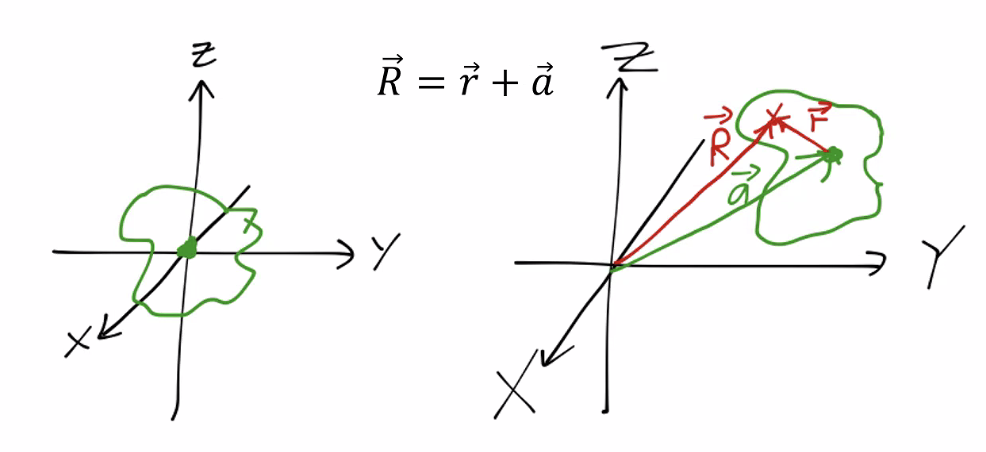
\includegraphics[scale=0.5]{Lecture-18/l18-img5.png}
\end{center}
If $I_{ij}$ is the inertia tensor calculated in the CM coordinates, and $J_{ij}$ is the tensor element in the displaced coordinates (where $\v{R} = \v{r} + \v{a}$), then:
\[J_{ij} = I_{ij} + M(a^2\delta_{ij} - a_ia_j)\]

\subsubsection{Example: Applying the Parallel Axis Theorem to the Cube}
For the displacement of coordinates from the center of the mass of the cube to the corner of the cube, we have that:
\[\v{a} = \m{-b/2 \\ -b/2 \\ -b/2}, \quad a^2 = \abs{\v{a}}^2 = \frac{3}{4}b^2\]
Then, for the diagonal elements we have:
\[M(a^2\delta_{ii} - a_ia_i) = M\left[\frac{3}{4}b^2 - \frac{-b}{2}\cdot\frac{-b}{2}\right] = \frac{Mb^2}{2}\]
And for the off diagonals:
\[M(a^2\delta_{ij} - a_ia_j) = M\left[-\frac{-b}{2}\frac{-b}{2}\right] = -\frac{Mb^2}{4}\]
Hence calculating the inertia tensor about the corner of the cube (in the displaced coordinates) we get:
\[\mathbb{J} = Mb^2\m{1/6 & 0 & 0 \\ 0 & 1/6 & 0 \\ 0 & 0 & 1/6} + Mb^2\m{1/2 & -1/4 & -1/4 \\ -1/4 & 1/2 & -1/4 \\ -1/4 & -1/4 & 1/2} = Mb^2\m{2/3 & -1/4 & -1/4 \\ -1/4 & 2/3 & -1/4 \\ -1/4 & -1/4 & 2/3}\]
Which agrees with the result obtained from the direct calculation.

\subsubsection{Principal axes}
If $\v{L} = \lambda\bm{\omega}$ for a scalar $\lambda$, the body rotates around one of its principal axes. $\lambda$ is the "Moment of inertia" about that axis. So if:
\[\II = \m{\lambda_1 & 0 & 0 \\ 0 & \lambda_2 & 0 \\ 0 & 0 & \lambda_3}\]
Then the chosen axes are the principal axes and $\lambda_i$ are the principal moments. For any rigid body and any point $O$, there are three perpendicular axes with respect to which the inertia tensor is diagonal! This is a consquence of the fact that the moment of inertia tensor has real entries and is symmetric. 
\newline Which of the following statements are a consequence of the fact that the inertia tensor is a 3x3 matrix with real positive eigenvalues and orthogonal eigenvectors?
\begin{enumerate}
    \item The matrix can be diagonalized
    \item The matrix of eigenvectors is an orthogonal matrix
    \item The matrix of eigenvectors is a rotation matrix (if properly normalized)
    \item In the coordinate system aligned with the eigenvectors, the tensor is diagonal.
\end{enumerate}
\begin{s}
    All 4 are correct. 
\end{s}